%\VignetteIndexEntry{flexsurv user guide}

\documentclass[nojss,nofooter]{jss}
\usepackage{bm}
\usepackage{tabularx}
\usepackage{graphics}

\author{Christopher H. Jackson \\ MRC Biostatistics Unit, Cambridge, UK \\ \email{chris.jackson@mrc-bsu.cam.ac.uk}}
\title{flexsurv: a platform for parametric survival modelling in R}

\Plainauthor{Christopher Jackson, MRC Biostatistics Unit}

\Abstract{ \pkg{flexsurv} is an R package for fully-parametric
  modelling of survival data.  Any parametric time-to-event
  distribution may be fitted if the user supplies at minimum a
  probability density or hazard function.  Many survival distributions
  are built in, including standard models models and the three and
  four-parameter generalized gamma and F distributions.  Any parameter
  of the distribution can be modelled as a linear or log-linear
  function of covariates.  Another built-in model is the spline model
  of Royston and Parmar, in which both baseline survival and covariate
  effects can be arbitrarily flexible parametric functions of time.
  The main model-fitting function, \code{flexsurvreg}, uses the
  familiar syntax of \code{survreg} from the standard \pkg{survival}
  package.  Censoring or left-truncation are specified in \code{Surv}
  objects.  Estimates and confidence intervals for any function of the
  model parameters can be printed or plotted.  \pkg{flexsurv} also
  enhances the \pkg{mstate} package \citep{mstate:jss} by providing
  cumulative hazards for fully-parametric multi-state models.  This
  article explains the methods and design principles of the package,
  giving several worked examples of its use.  } 

\Keywords{survival}

\usepackage{Sweave}
\begin{document}

\section{Motivation and design}

The Cox model for survival data is ubiquitous in medical research,
since the effects of predictors can be estimated without needing to
supply a baseline survival distribution that might be inaccurate.
However, fully-parametric models have many advantages, and even the
originator of the Cox model has expressed a preference for parametric
modelling \citep[see][]{reid:cox:conversation}.  Fully-specified
models help to understand the pattern of the change in hazard through
time, and help with prediction and extrapolation. For example, the
mean survival $E(T) = \int_0^{\infty}S(t)$, used in health economic
evaluations \citep{latimer2013survival}, needs the survivor function
$S(t)$ to be fully-specified for all times $t$.

%% Cox "That's right, but since then various people have shown that
%% the answers are very insensitive to the parametric
%% formulation of the underlying distribution. And if you want
%% to do things like predict the outcome for a particular patient,
%% it's much more convenient to do that parametrically."

\pkg{flexsurv} allows parametric distributions of
arbitrary complexity to be fitted to survival data, gaining the
convenience of parametric modelling, while avoiding the risk of model
misspecification.  Built-in choices include splines with any number of
knots \citep{royston:parmar} and 3--4 parameter generalized gamma and
F distribution families.  Any user-defined model may be employed by
supplying at minimum an R function to compute the probability density
or hazard, and ideally also its cumulative form.  Any parameters may
be modelled in terms of covariates, and any function of the parameters
may be printed or plotted in model summaries.

\pkg{flexsurv} is intended as a general platform for survival
modelling in R.  The \code{survreg} function in the R package
\pkg{survival} \citep{therneau:survival} only supports two-parameter
(location/scale) distributions, though users can supply their own
distributions if they can be parameterised in this form.  Many other
contributed R packages can fit survival models, e.g. \pkg{eha}
\citep{eha} and \pkg{VGAM} \citep{yee:wild}, though these are either
limited to specific distribution families, not specifically designed
for survival analysis, or \citep[\pkg{ActuDistns},][]{actudistns}
contain only the definitions of distribution functions.
\pkg{flexsurv} enables distribution functions provided by such
packages to be used as survival models.

It is similar in spirit to the Stata packages \pkg{stpm2}
\citep{stpm2} for spline-based survival modelling, and \pkg{stgenreg}
\citep{stgenreg} for fitting survival models with user-defined hazard
functions using numerical integration.  Though in \pkg{flexsurv},
numerical integration can be avoided if the analytic cumulative
distribution or hazard can be supplied, and optimisation can also be
speeded by supplying analytic derivatives.  \pkg{flexsurv} also has
features for multi-state modelling and interval censoring, and general
output reporting.  It employs functional programming to work with
user-defined or existing R functions.

\S\ref{sec:general} explains the general model that \pkg{flexsurv} is
based on.  \S\ref{sec:models} gives examples of its use for fitting
built-in survival distributions with a fixed number of parameters, and
\S\ref{sec:custom} explains how users can define new distributions.
\S\ref{sec:adim} concentrates on classes of models where the number of
parameters can be chosen by the user, such as splines.  In
\S\ref{sec:multistate} a simple use of \pkg{flexsurv} for parametric
multi-state modelling is described.  Finally \S\ref{sec:extensions}
suggests some potential future extensions.


\section{General parametric survival model}
\label{sec:general}

\subsection{Definitions} 

The general model that \pkg{flexsurv} fits has probability density function
\begin{equation}
  \label{eq:model}
  f(t | \mu(\mathbf{z}), \bm{\alpha}(\mathbf{z})), \quad t \geq 0  
\end{equation}

The cumulative distribution function $F(t)$, survivor
function $S(t) = 1 - F(t)$, cumulative hazard $H(t) = -\log S(t)$ and
hazard $h(t) = f(t)/S(t)$ are also defined (suppressing the conditioning for clarity).
$\mu=\alpha_0$ is the parameter of primary interest,
which usually governs the mean or \emph{location} of the distribution.  Other
parameters $\bm{\alpha} = \alpha_1, \ldots, \alpha_R$ are called
``ancillary'' and determine the shape, variance or higher moments.

%%% Covariates may be time-dependent, but this notation generalizes to left-truncation, ref msm section 

\paragraph{Covariates} 

All parameters may depend on a vector of covariates $\mathbf{z}$
through link-transformed linear models $g_0(\mu) = \gamma_0 + \bm{\beta}_0^{'}
\mathbf{z}$ and $g_r(\alpha_r) = \gamma_r + \bm{\beta}_r^{'} \mathbf{z}$. $g()$
will typically be $\log()$ if the parameter is defined to be positive,
or the identity function if the parameter is unrestricted.  

Suppose that the location parameter, but not the ancillary parameters, depends
on covariates.  If the hazard function factorises as $h(t | \alpha,
\mu(\mathbf{z})) = \mu(\mathbf{z}) h_0(t | \alpha)$, then this is a
\emph{proportional hazards} (PH) model, so that the hazard ratio between
two groups (defined by two different values of $\mathbf{z}$) is constant
over time.

Alternatively, if $S(t | \mu(\mathbf{z}), \alpha) =
S(\mu(\mathbf{z}) t | \alpha)$ then it is an \emph{accelerated
  failure time} (AFT) model, so that the effect of covariates is to speed or
slow the passage of time. For example, doubling the value of a
covariate with coefficient $\beta=\log(2)$ would give half the
expected survival time.


\paragraph{Data and likelihood} 

Let $t_i: i=1,\ldots, n$ be a sample of times from individuals $i$.
Let $c_i=1$ if $t_i$ is an observed death time, or $c_i=0$ if $t_i$ is
a right-censoring time, thus the true death time is known only to be
greater than $t_i$.  Also let $s_i$ be corresponding left-truncation
(or delayed-entry) times, meaning that individual $i$ is only observed
conditionally on having survived up to $s_i$, thus $s_i=0$ if there is
no left-truncation.  This facilitates time-dependent covariates
(\S\ref{sec:models}) and multi-state models (\S\ref{sec:multistate}).
Additionally let $t^{max}_i$ be left-censoring times, a less common situation.  If there is no
left-censoring then these are infinite, so that $S(t^{max}_i)=0$; or
if the $i$th death time is interval-censored then $c_i=0$ and
$t^{max}_i$ is finite.

The likelihood for the parameters $\bm{\theta} = \{\bm{\gamma},\bm{\beta}\}$ in model
(\ref{eq:model}), given the corresponding data vectors, is
\begin{equation}
  \label{eq:lik}
  l(\{\bm{\theta}\} | \mathbf{t},\mathbf{c},\mathbf{s},\mathbf{t}^{max}) = \left\{ \prod_{i:\ c_i=1} f_i(t_i) \prod_{i:\ c_i=0} \left(S_i(t_i) - S_i(t^{max}_i)\right)\right\} / \prod_i S_i(s_i)  
\end{equation}

The individuals are independent, so that \pkg{flexsurv} does not
currently support shared frailty, clustered or random effects models
(see \S\ref{sec:extensions}).

\section{Fitting standard parametric survival models} 
\label{sec:models}

An example dataset used throughout this paper is from 686 patients
with primary node positive breast cancer, available in the package as
\code{bc}. This was originally provided with \pkg{stpm}
\citep{stpm:orig}, and analysed in much more detail by
\citet{sauerbrei1999building} and \citet{royston:parmar}.  The first
two records are:
\begin{Schunk}
\begin{Sinput}
> bc[1:2,]
\end{Sinput}
\begin{Soutput}
  censrec rectime group   recyrs
1       0    1342  Good 3.676712
2       0    1578  Good 4.323288
\end{Soutput}
\end{Schunk}
The main model-fitting function is called \code{flexsurvreg}.  Its
first argument is an R \emph{formula} object.  The left hand side of
the formula gives the response as a survival object, using the
\code{Surv} function from the \pkg{survival} package.  Here, this
indicates that the response variable is \code{recyrs}. 
This represents time of death or cancer recurrence when \code{censrec} is 1, 
or censoring when \code{censrec} is 0.  The covariate \code{group} is
a factor representing a prognostic score, with three levels
\code{"Good"} (the baseline), \code{"Medium"} and
\code{"Poor"}. All of these variables are in the data frame
\code{bc}.
\begin{Schunk}
\begin{Sinput}
> library(flexsurv)
> fs1 <- flexsurvreg(Surv(recyrs, censrec) ~ group, data=bc, dist="weibull")
\end{Sinput}
\end{Schunk}
If the argument \code{dist} is a string, this denotes a built-in
survival distribution.  In this case we fit a Weibull survival model.

Printing the fitted model object gives estimates and confidence
intervals for the model parameters and other useful information.  Note
that these are the \emph{same parameters} as represented by the R
distribution function \code{dweibull}: the \code{shape} $\alpha$ and
the \code{scale} $\mu$ of the survivor function $S(t) =
\exp(-(t/\mu)^\alpha)$, and \code{group} has a linear effect on
$\log(\mu)$.
\begin{Schunk}
\begin{Sinput}
> fs1
\end{Sinput}
\begin{Soutput}
Call:
flexsurvreg(formula = Surv(recyrs, censrec) ~ group, data = bc,     dist = "weibull")

Estimates: 
             data mean  est      L95%     U95%     se       exp(est)  L95%   
shape             NA     1.3797   1.2548   1.5170   0.0668       NA        NA
scale             NA    11.4229   9.1818  14.2110   1.2728       NA        NA
groupMedium   0.3338    -0.6136  -0.8623  -0.3649   0.1269   0.5414    0.4222
groupPoor     0.3324    -1.2122  -1.4583  -0.9661   0.1256   0.2975    0.2326
             U95%   
shape             NA
scale             NA
groupMedium   0.6943
groupPoor     0.3806

N = 686,  Events: 299,  Censored: 387
Total time at risk: 2113.425
Log-likelihood = -811.9419, df = 4
AIC = 1631.884
\end{Soutput}
\end{Schunk}
The same model can be fitted using \code{survreg} in 
\pkg{survival}:
\begin{Schunk}
\begin{Sinput}
> survreg(Surv(recyrs, censrec) ~ group, data=bc, dist="weibull")
\end{Sinput}
\begin{Soutput}
Call:
survreg(formula = Surv(recyrs, censrec) ~ group, data = bc, dist = "weibull")

Coefficients:
(Intercept) groupMedium   groupPoor 
  2.4356168  -0.6135892  -1.2122137 

Scale= 0.7248206 

Loglik(model)= -811.9   Loglik(intercept only)= -873.2
	Chisq= 122.53 on 2 degrees of freedom, p= 0 
n= 686 
\end{Soutput}
\end{Schunk}
The maximised log-likelihoods are the same, however the
parameterisation is different: the first coefficient
\code{(Intercept)} reported by \code{survreg} is $\log(\mu)$, and
\code{survreg}'s \code{"scale"} is \code{dweibull}'s (thus
\code{flexsurvreg})'s 1 / \code{shape}. The covariate effects
$\bm{\beta}$, however, have the same ``accelerated failure time''
interpretation, as linear effects on $\log(\mu)$.  The multiplicative
effects $\exp(\bm{\beta})$ are printed in the output as
\code{exp(est)}.

\paragraph{Alternative censoring or truncation mechanisms} 

If we also had left-truncation times in a variable called
\code{start}, the response would be 
\code{Surv(start,recyrs,censrec)}.  Or if all responses were
interval-censored between lower and upper bounds \code{tmin} and
\code{tmax}, then we would write
\code{Surv(tmin,tmax,type="interval2")}.  

Note that just as in \texttt{survreg}, time-dependent covariates can
be represented in ``counting process'' form --- as a series of
left-truncated survival times.  For each individual there would be
multiple records, each corresponding to an interval where the
covariate is assumed to be constant.  The response would be of the
form \code{Surv(start,stop,censrec)}, where \code{start} and
\code{stop} are the limits of each interval, and \code{censrec}
indicates whether a death was observed at \code{stop}.  The function
\code{survSplit} in \pkg{survival} is a utility to construct data like
this.


\subsection{Built-in models}

\code{flexsurvreg}'s currently built-in distributions are listed in
Table \ref{tab:dists}.  In each case, the probability density $f()$
and parameters of the fitted model are taken from an existing R
function of the same name but beginning with the letter \code{d}.  For
the Weibull, exponential (\code{dexp}), gamma (\code{dgamma}) and
log-normal (\code{dlnorm}), the density functions are provided with
standard installations of R.  These density functions, and the
corresponding cumulative distribution function (with first letter
\code{p} instead of \code{d}) are used internally in
\code{flexsurvreg} to compute the likelihood.

\pkg{flexsurv} provides some additional survival distributions,
including a Gompertz distribution with unrestricted shape parameter
(\code{dist="gompertz"}), and the three- and four-parameter families
described below.  For all built-in distributions, \pkg{flexsurv} also
defines functions beginning \code{h} giving the hazard, and \code{H}
for cumulative hazard.

\paragraph{Generalized gamma} This three-parameter distribution
includes the Weibull, gamma and log-normal as special cases.  The
original parameterisation from \citet{stacy:gengamma} is available as\\
\code{dist="gengamma.orig"}, however the newer parameterisation
\citep{prentice:loggamma} is preferred: \code{dist="gengamma"}.  This has
parameters ($\mu$,$\sigma$,$q$), and survivor function
\[
\begin{array}{ll}
1 - I(\gamma,u)   & (q > 0)\\
1 - \Phi(z)  & (q = 0)\\
\end{array}
\]
where $I(a,x) = \int_0^x x^{a-1}\exp(-x)/\Gamma(a)$ is the incomplete gamma function (the cumulative gamma distribution with shape $a$ and scale 1), $\Phi$ is the standard normal cumulative distribution,  $u = \gamma \exp(|q|z)$, $z=(\log(t) - \mu)/\sigma$, and $\gamma=q^{-2}$.   The \citet{prentice:loggamma} parameterisation extends the original one to include a further class of models with negative $q$, and survivor function $I(\gamma,u)$, where $z$ is replaced by $-z$.   This stabilises estimation when the distribution is close to log-normal, since $q=0$ is no longer near the boundary of the parameter space.    In R notation, \footnote{The parameter called $q$ here and in previous literature is called $Q$ in \code{dgengamma} and related functions, since the first argument of a cumulative distribution function is conventionally named \code{q}, for quantile, in R.} the parameter values corresponding to the three special cases are

\begin{Code}
dgengamma(x, mu, sigma, Q=0)     ==  dlnorm(x, mu, sigma)                                
dgengamma(x, mu, sigma, Q=1)     ==  dweibull(x, shape=1/sigma, scale=exp(mu))           
dgengamma(x, mu, sigma, Q=sigma) ==  dgamma(x, shape=1/sigma^2, 
                                               rate=exp(-mu) / sigma^2)  
\end{Code}

The generalized gamma model is fitted to the breast cancer survival
data. \code{fs2} is an AFT model, where only the parameter
$\mu$ depends on the prognostic covariate \code{group}.  In a second
model \code{fs3}, the first ancillary parameter \code{sigma} ($\alpha_1$) also
depends on this covariate, giving a model with a time-dependent effect
that is neither PH nor AFT.  The second ancillary parameter \code{Q}
is still common between prognostic groups.
\begin{Schunk}
\begin{Sinput}
> fs2 <- flexsurvreg(Surv(recyrs, censrec) ~ group, data=bc, dist="gengamma")
> fs3 <- flexsurvreg(Surv(recyrs, censrec) ~ group + sigma(group), 
+                    data=bc, dist="gengamma")
\end{Sinput}
\end{Schunk}
Table \ref{tab:aic} compares all the models fitted to the breast
cancer data, showing absolute fit to the data as measured by the
maximised -2$\times$ log likelihood $-2LL$, number of parameters $p$,
and Akaike's information criterion $-2LL + 2p$ which estimates
predictive ability.


\paragraph{Generalized F} This four-parameter distribution includes
the generalized gamma, and also the log-logistic, as special cases.
The variety of hazard shapes that can be represented is discussed by
\citet{ccox:genf}.  It is provided here in alternative ``original''
(\code{dist="genf.orig"}) and ``stable'' parameterisations
(\code{dist="genf"}) as presented by \citet{prentice:genf}. 
See \code{help(GenF)} and \code{help(GenF.orig)} in the package documentation 
for the exact definitions.


\begin{table}
  \begin{tabular}{llll}
\hline
    &  Parameters &  Density R function & \code{dist}\\
\hline
    Exponential & \code{rate}             & \code{dexp}   & \code{"exp"} \\
    Weibull     & \code{shape, scale}     & \code{dweibull} & \code{"weibull"} \\
    Gamma       & \code{shape, rate}      & \code{dgamma} & \code{"gamma"}\\
    Log-normal  & \code{meanlog, sdlog}   & \code{dlnorm} & \code{"lnorm"}\\
    Gompertz    & \code{shape, rate}      & \code{dgompertz} & \code{"gompertz"} \\
    Generalized gamma (Prentice 1975)   & \code{mu, sigma, Q} & \code{dgengamma} & \code{"gengamma"} \\
    Generalized gamma (Stacy 1962)& \code{shape, scale, k} & \code{dgengamma.orig} & \code{"gengamma.orig"} \\
    Generalized F     (stable)    & \code{mu, sigma, Q, P} & \code{dgenf} & \code{"genf"} \\
    Generalized F     (original)  & \code{mu, sigma, s1, s2} & \code{dgenf.orig} & \code{"genf.orig"} \\
\hline
  \end{tabular}
  \caption{Built-in parametric survival distributions in \pkg{flexsurv}}
  \label{tab:dists}
\end{table}

\subsection{Plotting outputs}
\label{sec:plots}

The \code{plot()} method for \code{flexsurvreg} objects is used as a
quick check of model fit.  By default, this draws a Kaplan-Meier
estimate of the survivor function $S(t)$, one for each combination of
categorical covariates, or just a single ``population average'' curve if there are no
categorical covariates (Figure \ref{fig:surv}).  The corresponding estimates from the fitted
model are overlaid.  Fitted values from further models can be added
with the \code{lines()} method.  
\begin{figure}[h]
  \centering
\begin{Schunk}
\begin{Sinput}
> plot(fs1, col="gray", lwd.obs=2, xlab="Years", ylab="Recurrence-free survival")
> lines(fs2, col="red", lty=2)
> lines(fs3, col="red")
> legend("bottomleft", col=c("black","gray","red","red"), 
+        lty=c(1,1,2,1), bty="n", lwd=rep(2,4),
+        c("Kaplan-Meier","Weibull","Generalized gamma (AFT)",
+          "Generalized gamma (time-varying"))
\end{Sinput}
\end{Schunk}
\includegraphics{flexsurv-006}
  \caption{Estimated survival from parametric models and Kaplan-Meier estimates.}
  \label{fig:surv}
\end{figure}

\code{scale="hazard"} can be used to plot hazards from parametric
models against kernel density estimates obtained from \pkg{muhaz}
\citep{muhaz,mueller:wang}. Figure \ref{fig:haz} shows more clearly why the Weibull
model is inadequate: the hazard must be increasing or decreasing ---
while the generalized gamma can represent the increase and subsequent
decline in hazard seen in the data.   Similarly, \code{scale="cumhaz"} plots cumulative hazards. 
\begin{figure}[h]
  \centering
\begin{Schunk}
\begin{Sinput}
> plot(fs1, type="hazard", col="gray", lwd.obs=2, xlab="Years", ylab="Hazard")
> lines(fs2, type="hazard", col="red", lty=2)
> lines(fs3, type="hazard", col="red")
> legend("topright", col=c("black","gray","red","red"),
+        lty=c(1,1,2,1),  bty="n", lwd=rep(2,4),
+        c("Kernel density estimate","Weibull","Gen. gamma (AFT)","Gen. gamma (time-varying)"))
\end{Sinput}
\end{Schunk}
\includegraphics{flexsurv-007}
  \caption{Estimated hazards from parametric models and kernel density estimates.}
  \label{fig:haz}
\end{figure}

The numbers plotted are available from the
\code{summary.flexsurvreg()} method.  Confidence intervals are
produced by simulating a large sample from the asymptotic normal
distribution of the maximum likelihood estimates of $\{\bm{\beta}_r:
r=0,\ldots,R$, via the function \code{normboot.flexsurvreg}.

In this example, there is only a single categorical covariate, and the
\code{plot} and \code{summary} methods return one observed and fitted
trajectory for each level of that covariate.  For more complicated
models, users should specify what covariate values they
want summaries for, rather than relying on the default \footnote{If there are only factor covariates, all combinations are plotted.  If
there are any continuous covariates, these methods by default return a ``population average''
curve, with the linear model design matrix set to its average
values, including the 0/1 contrasts defining factors, which doesn't
represent any specific covariate combination.}.
This is done by supplying the \code{newdata} argument, a 
data frame or list containing covariate values, just as
in standard R functions like \code{predict.lm}.

This \code{plot()} method is only for casual exploratory use.  For
publication-standard figures, it is preferable to set up the axes
beforehand, and use the \code{lines()} method, or construct plots by
hand using the data available from \code{summary.flexsurvreg()}.



\subsection{Custom model summaries}

Any function of the parameters of a fitted model can be summarised or plotted by
supplying the argument \code{fn} to \code{summary.flexsurvreg} or
\code{plot.flexsurvreg}.  This should be an R function, with mandatory
first two arguments \code{t} representing time, and \code{start}
representing a left-truncation point (so that the result is
conditional on survival up to that time). The remaining arguments must
be the parameters of the survival distribution.  For example, median 
survival under the Weibull model \code{fs1} can be summarised as follows
\begin{Schunk}
\begin{Sinput}
> median.weibull <- function(t, start, shape, scale) { 
+     qweibull(0.5, shape=shape, scale=scale) 
+ }
> summary(fs1, fn=median.weibull, t=1, B=10000)
\end{Sinput}
\begin{Soutput}
group=Good 
  time     est      lcl      ucl
1    1 8.75794 7.084824 10.75859

group=Medium 
  time      est      lcl      ucl
1    1 4.741585 4.106784 5.448722

group=Poor 
  time      est     lcl      ucl
1    1 2.605819 2.31059 2.929204
\end{Soutput}
\end{Schunk}
Although the median of the Weibull has an analytic form as $\mu
\log(2)^{1/\alpha}$, the form of the code given here generalises to
other distributions.
The argument \code{t} is not used in \code{median.weibull}, because
the median is a time-constant function of the parameters, unlike the
survival or hazard.

\code{10000} random samples are drawn to produce
a slightly more precise confidence interval than the default --- users
should adjust this until the desired level of precision is obtained.
A useful future extension of the package would be to allow users to 
supply derivatives of their custom summary function, so that the 
delta method can be used to obtain approximate confidence intervals 
without simulation.


\subsection{Computation}

The likelihood is maximised in \code{flexsurvreg} using the
optimisation methods available through the standard R \code{optim}
function.  By default, this is the \code{"BFGS"} method \citep{nash}
using the analytic derivatives of the likelihood with respect to the
model parameters, if these are available, to improve the speed of
convergence to the maximum.  These are built-in for the exponential,
Weibull and Gompertz, and the hazard- and odds-based spline models
(see \S\ref{sec:spline}).  For custom distributions (see
\S\ref{sec:custom}), the user can optionally supply functions with
names beginning \code{"DLd"} and \code{"DLS"} respectively
(e.g. \code{DLdweibull,DLSweibull}) to calculate the derivatives of
the log density and log survivor functions with respect to the
transformed baseline parameters $\gamma$.


\section{Custom survival distributions}
\label{sec:custom}

\pkg{flexsurv} is not limited to its built-in distributions.  Any
survival model of the form (\ref{eq:model}--\ref{eq:lik}) can be
fitted if we can provide either the density function $f()$ or the
hazard $h()$.  Many contributed R packages provide probability density
and cumulative distribution functions for positive distributions.  
Though survival models may be more naturally characterised by their
hazard function, representing the changing risk of death through time.
For example, for survival following major surgery we may want a
``U-shaped'' hazard curve, representing a high risk soon after the
operation, which then decreases, but increases naturally as survivors
grow older.

To supply a custom distribution, the \code{dist} argument to
\code{flexsurvreg} is defined to be an R list object, rather than a
character string.  The list has the following elements.

\begin{description}
\item[\code{name}] Name of the distribution.  For example, if this is \code{"llogis"} then there is assumed to be at least either 
  
  \begin{itemize}
  \item  a function called \code{dllogis} to compute the probability density, or 
  \item \code{hllogis} to compute the hazard.  
  \end{itemize}
  
  Ideally there will also be a function called \code{pllogis} for the
  cumulative distribution (if \code{d} is given), or \code{H} for the
  cumulative hazard (to complement \code{h}).  If there is no analytic
  form for $F(t)$ or $H(t)$, then \pkg{flexsurv} can compute these
  internally by numerical integration, as in \pkg{stgenreg}
  \citep{stgenreg}.  The default options of the built-in R routine
  \code{integrate} for adaptive quadrature are used, though these may
  be changed using the \code{integ.opts} argument to
  \code{flexsurvreg}.  Models specified this way will take an order of
  magnitude more time to fit, and the fitting procedure may be unstable.
  An example is given in \S\ref{sec:gdim}.
  
  These functions must be \emph{vectorised}, and the density function
  must also accept an argument \code{log}, which when \code{TRUE},
  returns the log density.  See the examples below.
  
\item[\code{pars}] Character vector naming the parameters of the
  distribution $\mu,\alpha_1,...,\alpha_R$.  These must match the
  arguments of the R distribution function or functions.
  
\item[\code{location}] Character: quoted name of the location parameter $\mu$.
  The location parameter will not necessarily be the first one, e.g. 
  in \code{dweibull} the \code{scale} comes after the \code{shape}.
  
\item[\code{transforms}] A list of functions $g()$ which transform the parameter from its natural range to the real line, for example, \code{c(log,identity)} \footnote{This is a \emph{list}, not an \emph{atomic vector} of functions, so if the distribution only has one parameter, we should write \code{transforms=c(log)} or \code{transforms=list(log)}, not \code{transforms=log}}

\item[\code{inv.transforms}] List of corresponding inverse functions.

\item[\code{inits}] A function which provides plausible initial values
  of the parameters for maximum likelihood estimation.  This is
  optional, but if not provided, then each call to \code{flexsurvreg}
  must have an \code{inits} argument containing a vector of initial
  values, which is inconvenient.  Implausible initial values may
  produce a likelihood of zero, and a fatal error message
  (\texttt{initial value in `vmmin' is not finite}) from the
  optimiser.
  
  Each distribution will ideally have a heuristic for initialising
  parameters from summaries of the data.  For example, since the
  median of the Weibull is $\mu \log(2)^{1/\alpha}$, a sensible
  estimate of $\mu$ will commonly be the median log uncensored
  survival time divided by $\log(2)$, with $\alpha=1$, assuming that
  in practice the true value of $\alpha$ is not often far from 1.  Then
  we define the function, of one argument \code{t} assumed to be the
  uncensored survival times, returning the initial values for the
  Weibull \code{shape} and \code{scale} respectively.

  \code{inits = function(t){ c(1, median(t[t>0]) / log(2)) } }
  
  More complicated initial value functions may use other data such
  as the covariate values and censored observations: for an example,
  see the function \code{flexsurv.splineinits} in the package source
  that computes initial values for spline models
  (\S\ref{sec:spline}).

\end{description}
    
\paragraph{Example: Using functions from a contributed package}

The following custom model uses the log-logistic distribution functions
(\code{dllogis} and \code{pllogis}) available in the package
\pkg{eha}.   The survivor function is $S(t|\mu,\alpha) = 1/(1 + (t/\mu)^\alpha)$,
so that the odds $(1-S(t))/S(t)$ of having died are a linear function of log time.
\begin{Schunk}
\begin{Sinput}
> library(eha)
> custom.llogis <- list(name="llogis",  pars=c("shape","scale"), location="scale",
+                       transforms=c(log, log), inv.transforms=c(exp, exp),
+                       inits=function(t){ c(1, median(t)) })
> fs4 <- flexsurvreg(Surv(recyrs, censrec) ~ group, data=bc, dist=custom.llogis)
\end{Sinput}
\end{Schunk}

This fits the breast cancer data better than the Weibull, since it can
represent a peaked hazard, but less well than the generalized gamma (Table \ref{tab:aic}).


\paragraph{Example: Wrapping functions from a contributed package}

Sometimes there may be probability density and similar functions in a
contributed package, but in a different format.  For example,
\pkg{eha} also provides a three-parameter Gompertz-Makeham
distribution with hazard $h(t|\mu,\alpha_1,\alpha_2)= \alpha_2 + \alpha_1 \exp(t/\mu)$.
The shape parameters $\alpha_1,\alpha_2$ are provided to 
\code{dmakeham} as a vector argument of length two.  However, \code{flexsurvreg}
expects distribution functions to have one argument for each
parameter.  Therefore we write our own functions that wrap around 
the third-party functions.
\begin{Schunk}
\begin{Sinput}
> dmakeham3 <- function(x, shape1, shape2, scale, ...)  {
+     dmakeham(x, shape=c(shape1, shape2), scale=scale, ...)
+ }
> pmakeham3 <- function(q, shape1, shape2, scale, ...)  {
+     pmakeham(q, shape=c(shape1, shape2), scale=scale, ...)
+ }
\end{Sinput}
\end{Schunk}
\code{flexsurvreg} also requires these functions to be
\emph{vectorized}, as the standard distribution functions in R are.
That is, we can supply a vector of alternative values for one or more
arguments, and expect a vector of the same length to be returned.  The
R base function \code{Vectorize} can be used to do this here.
\begin{Schunk}
\begin{Sinput}
> dmakeham3 <- Vectorize(dmakeham3) 
> pmakeham3 <- Vectorize(pmakeham3)
\end{Sinput}
\end{Schunk}
and this allows us to write, for example, 
\begin{Schunk}
\begin{Sinput}
> pmakeham3(c(0, 1, 1, Inf), 1, c(1, 1, 2, 1), 1)
\end{Sinput}
\begin{Soutput}
[1] 0.0000000 0.9340120 0.9757244 1.0000000
\end{Soutput}
\end{Schunk}
We could then use \code{dist=list(name="makeham3", pars=c("shape1","shape2","scale"),...)}
in a \code{flexsurvreg} model, though in the breast cancer example,
the second shape parameter is poorly identifiable.


\paragraph{Example: Changing the parameterisation of a distribution}

We may want to fit a Weibull model like \code{fs1}, but parameterised as $S(t) =
\exp(-\mu t^\alpha)$, so that the covariate effects reported in the
printed \code{flexsurvreg} object can be interpreted as hazard ratios
or log hazard ratios without any further transformation.
Here instead of the density and cumulative distribution functions, we
provide the hazard and cumulative hazard.\footnote{The \pkg{eha} package 
needs to be detached first so that \pkg{flexsurv}'s built-in \code{hweibull} is used, which returns \code{NaN} if the parameter values are zero, rather than failing as \pkg{eha}'s does.}
\begin{Schunk}
\begin{Sinput}
> detach("package:eha")
> hweibullPH <- function(x, shape, scale = 1, log=FALSE){
+     hweibull(x, shape=shape, scale=scale^{-1/shape}, log=log)
+ }
> HweibullPH <- function(x, shape, scale=1, log=FALSE){
+     Hweibull(x, shape=shape, scale=scale^{-1/shape}, log=log)
+ }
> custom.weibullPH <- list(name="weibullPH", 
+                          pars=c("shape","scale"), location="scale",
+                          transforms=c(log, log), inv.transforms=c(exp, exp),
+                          inits = function(t){
+                              c(1, median(t[t>0]) / log(2))
+                          })
> fs6 <- flexsurvreg(Surv(recyrs, censrec) ~ group, data=bc, dist=custom.weibullPH)
> 1 / fs1$res["scale","est"]^fs1$res["shape","est"]
\end{Sinput}
\begin{Soutput}
[1] 0.03472474
\end{Soutput}
\begin{Sinput}
> 1 / exp(fs1$res["groupMedium","est"]) ^ fs1$res["shape","est"]
\end{Sinput}
\begin{Soutput}
[1] 2.331564
\end{Soutput}
\end{Schunk}
The fitted model is the same as \code{fs1}, therefore the maximised likelihood is the same,
and the parameter estimates of \code{fs1} can be transformed to those of \code{fs6} as shown.

A slightly more complicated example is given in the package vignette
\code{flexsurv-examples} of constructing a proportional hazards
generalized gamma model.





\section{Arbitrary-dimension models}
\label{sec:adim}

\pkg{flexsurv} also supports models where the number of parameters is
arbitrary.  In the models discussed previously, the number of
parameters in the model family is fixed (e.g. three for the
generalized gamma).  In this section, the model complexity can be
chosen by the user, given the model family.  We may want to represent
more irregular hazard curves by more flexible functions, or use bigger
models if a bigger sample size makes it feasible to estimate more
parameters.


\subsection{Royston and Parmar spline model}
\label{sec:spline}

In the spline-based survival model of \citet{royston:parmar}, a
transformation $g(S(t,z))$ of the survival function is modelled as a
natural cubic spline function of log time, $x = \log(t)$, plus linear
effects of covariates $z$.  This is available here as the function
\code{flexsurvspline},  and is also available in the Stata package
\pkg{stpm2} \citep{stpm2} (and historically \pkg{stpm}, \citet{stpm:orig,stpm:update}).

  \[g(S(t,z)) = s(x, \bm{\gamma})\]

Typically we use $g(S(t,\mathbf{z}) = \log(-\log(S(t,\mathbf{z}))) =
\log(H(t,\mathbf{z}))$, the log cumulative hazard, giving a
proportional hazards model.    

\paragraph{Spline parameterisation}
The complexity of the model, thus the dimension of $\bm{\gamma}$, is
governed by the number of \emph{knots} $m$ in the spline function
$s()$.  Natural cubic splines are piecewise cubic polynomials defined
to be continuous, with continuous first and second derivatives at the
knots, and also constrained to be linear beyond boundary knots
$k_{min},k_{max}$.  As well as the boundary knots there may be up to
$m\geq 0$ \emph{internal} knots $k_1,\ldots k_m$.  Various spline
parameterisations exist --- the one used here is from
\citet{royston:parmar}.
\begin{equation}
  \label{eq:spline}
  s(x,\bm{\gamma}) = \gamma_0 + \gamma_1 x + \gamma_2 v_1(x) + \ldots + \gamma_{m+1} v_m(x)   
\end{equation}
where $v_j(x)$ is the $j$th \emph{basis} function

\[v_j(x) = (x - k_j)^3_+ - \lambda_j(x - k_{min})^3_+ - (1 - \lambda_j) (x - k_{max})^3_+, 
\qquad
\lambda_j = \frac{k_{max} - k_j}{k_{max} - k_{min}} \] 

and $(x - a)_+ = max(0, x - a)$.  If $m=0$ then there are only two
parameters $\gamma_0,\gamma_1$.  In fact if $g()$ is the log
cumulative hazard, this is equivalent to a Weibull model.  Table
\ref{tab:spline} explains two further choices of $g()$, and the
parameter values and distributions they simplify to for $m=0$.  
The probability density and cumulative distribution functions
for this model are available as \code{dsurvspline} and \code{psurvspline}.

  \begin{table}
  \begin{tabularx}{\textwidth}{lXlp{1.4in}}
\hline
    Model &  $g(S(t,\mathbf{z}))$ & In \code{flexsurvspline} & With $m=0$ \\
\hline
Proportional hazards
& $\log(-\log(S(t,\mathbf{z})))$ \newline {\footnotesize (log cumulative hazard)}
& \code{scale="hazard"}
& Weibull  {\footnotesize \code{shape} $\gamma_1$, \code{scale} $\exp(-\gamma_0/\gamma_1)$}\\
Proportional odds
& $\log(S(t,\mathbf{z})^{-1} - 1)$ \newline {\footnotesize (log cumulative odds)}
& \code{scale="odds"}
& Log-logistic  {\footnotesize \code{shape} $\gamma_1$, \code{scale} $\exp(-\gamma_0/\gamma_1)$}\\
Normal / probit
& $\Phi^{-1}(S(t,\mathbf{z}))$  \newline   {\footnotesize (inverse normal CDF, \code{qnorm})}
& \code{scale="normal"}
& Log-normal {\footnotesize \code{meanlog} $-\gamma_0/\gamma_1$, \code{sdlog} $1/\gamma_1$ }\\  
\hline
  \end{tabularx}    
  \caption{Alternative modelling scales for \code{flexsurvspline}, and equivalent distributions for $m=0$ (with parameter definitions as in the R \code{d} functions referred to elsewhere in the paper)}
    \label{tab:spline}
\end{table}

\paragraph{Covariates on spline parameters}
Covariates can be placed on any parameter $\gamma$ through a linear
model (with identity link function).  Most straightforwardly, we can
let the intercept $\gamma_0$ vary with covariates $\mathbf{z}$, giving
a proportional hazards or odds model (depending on $g()$).

\[g(S(t,z)) = s(x, \bm{\gamma}) + \bm{\beta}^T \mathbf{z} \]


The spline coefficients $\gamma_j: j=1, 2 \ldots$, the "ancillary parameters",
may also be modelled as linear functions of covariates $\mathbf{z}$, as

\[\gamma_j(\mathbf{z}) = \gamma_{j0} + \gamma_{j1}z_1 + \gamma_{j2}z_2 + \ldots\]

giving a model where the effects of covariates are arbitrarily flexible
functions of time: a non-proportional hazards or odds model.

\paragraph{Spline models in \pkg{flexsurv}}

The package provides the function \code{flexsurvspline} to fit this
general model. Internal knots are chosen by default from quantiles of
the log uncensored death times, or users can supply their own
knot locations in the \code{knots} argument to \code{flexsurvspline}.
Initial values for numerical likelihood maximisation are chosen using
the method described by \citet{royston:parmar} of Cox regression
combined with transforming an empirical survival estimate.

For example, the best-fitting model for the breast cancer dataset identified in \citet{royston:parmar},
a proportional odds model with one internal spline knot, is
\begin{Schunk}
\begin{Sinput}
> sp1 <- flexsurvspline(Surv(recyrs, censrec) ~ group, data=bc, k=1, 
+                       scale="odds")
\end{Sinput}
\end{Schunk}
A further model where the first ancillary parameter also depends on the prognostic
group, giving a time-varying odds ratio, is fitted as
\begin{Schunk}
\begin{Sinput}
> sp2 <- flexsurvspline(Surv(recyrs, censrec) ~ group + gamma1(group),
+                       data=bc, k=1, scale="odds")
\end{Sinput}
\end{Schunk}
These models give qualitatively similar results to the generalized
gamma in this dataset (Figure \ref{fig:spline:haz}), and have similar
predictive ability as measured by AIC (Table \ref{tab:aic}). Though in
general, an advantage of spline models is that extra flexibility is
available where necessary.
\begin{figure}[h]
  \centering
\begin{Schunk}
\begin{Sinput}
> plot(sp1, type="hazard", ylim=c(0, 0.5), xlab="Years", ylab="Hazard")
> lines(sp2, type="hazard", col="red", lty=2)
> lines(fs2, type="hazard", col="blue")
> legend("topright", c("black","red","red","blue"), lty=c(1,1,2,1), lwd=rep(2,4),
+        c("Kernel density estimate","Spline (proportional odds)",
+          "Spline (time-varying)","Generalized gamma (time-varying)"))
\end{Sinput}
\end{Schunk}
\includegraphics{flexsurv-016}
  \caption{Comparison of spline and generalized gamma fitted hazards}
  \label{fig:spline:haz}
\end{figure}
Note that the log hazard ratios under the proportional hazards spline
model are practically the same as under a standard Cox model.
\begin{Schunk}
\begin{Sinput}
> sp3 <- flexsurvspline(Surv(recyrs, censrec) ~ group, data=bc, k=1, scale="hazard")
> sp3$res[c("groupMedium","groupPoor"),c("est","se")]
\end{Sinput}
\begin{Soutput}
                  est        se
groupMedium 0.8334517 0.1712042
groupPoor   1.6111788 0.1640933
\end{Soutput}
\begin{Sinput}
> cox3 <- coxph(Surv(recyrs, censrec) ~ group, data=bc)
> coef(summary(  cox3))[,c("coef","se(coef)")]
\end{Sinput}
\begin{Soutput}
                 coef  se(coef)
groupMedium 0.8401002 0.1713926
groupPoor   1.6180720 0.1645443
\end{Soutput}
\end{Schunk}


\begin{Schunk}
\begin{Sinput}
> res <- t(sapply(list(fs1, fs2, fs3, fs4, sp1, sp2), 
+                 function(x)rbind(-2*x$loglik, x$npars, x$AIC)))
> rownames(res) <- c("Weibull","Generalized gamma",
+                    "Generalized gamma (time-varying effects)","Log-logistic",
+                    "Spline (sp1)", "Spline (sp2: time-varying effects)")
> colnames(res) <- c("-2 log likelihood","Parameters","AIC")
\end{Sinput}
\end{Schunk}
\begin{table}[h]
\begin{Schunk}
\begin{Sinput}
> res
\end{Sinput}
\begin{Soutput}
                                         -2 log likelihood Parameters      AIC
Weibull                                           1623.884          4 1631.884
Generalized gamma                                 1575.137          5 1585.137
Generalized gamma (time-varying effects)          1572.434          7 1586.434
Log-logistic                                      1598.105          4 1606.105
Spline (sp1)                                      1577.964          5 1587.964
Spline (sp2: time-varying effects)                1574.848          7 1588.848
\end{Soutput}
\end{Schunk}
  \caption{Comparison of parametric survival models fitted to the breast cancer data}
  \label{tab:aic}
\end{table}


\subsection{Implementing new general-dimension models}
\label{sec:gdim}

The spline model above is an example of the general parametric form
(\ref{eq:model}), but the number of parameters, $R+1$ in
(\ref{eq:model}), $m+2$ in (\ref{eq:spline}), is arbitrary.
\pkg{flexsurv} has the tools to deal with any model of this form.
\code{flexsurvspline} works internally by building a custom
distribution and then calling \code{flexsurvreg}.  Similar models may
in principle be built by users using the same method.  This relies on
a functional programming trick.

\paragraph{Creating distribution functions dynamically}

The R distribution functions supplied to custom models are expected to
have a fixed number of arguments, including one for each scalar
parameter.  However, the distribution functions for the spline model
(e.g. \code{dsurvspline}) have an argument \code{gamma} representing
the vector of parameters $\gamma$, whose length is determined by the
user through the choice of the number of knots.  Just as the
\emph{scalar parameters} of conventional distribution functions can be
supplied as \emph{vector arguments} (as explained in
\S\ref{sec:custom}), similarly, the vector parameters of spline-like
distribution functions can be supplied as \emph{matrix arguments},
representing alternative parameter values.

To convert a spline-like distribution function into the correct form,
\pkg{flexsurv} provides the utility \code{unroll.function}.  This
converts a function with one (or more) vector parameters (matrix
arguments) to a function with an arbitrary number of scalar parameters
(vector arguments).  For example, the 5-year survival probability for the baseline group 
under the model \code{sp1} is
\begin{Schunk}
\begin{Sinput}
> gamma <- sp1$res[c("gamma0","gamma1","gamma2"),"est"]
> 1 - psurvspline(5, gamma=gamma, knots=sp1$knots)
\end{Sinput}
\begin{Soutput}
[1] 0.6896969
\end{Soutput}
\end{Schunk}
An alternative function to compute this can be built by \code{unroll.function}.  We tell it that the 
vector parameter \code{gamma} should be provided instead as three scalar parameters
named \code{gamma0},\code{gamma1},\code{gamma2}.  The resulting function \code{pfn}
is in the correct form for a custom \code{flexsurvreg} distribution.
\begin{Schunk}
\begin{Sinput}
> pfn <- unroll.function(psurvspline, gamma=0:2)
> 1 - pfn(5, gamma0=gamma[1], gamma1=gamma[2], gamma2=gamma[3], knots=sp1$knots)
\end{Sinput}
\begin{Soutput}
[1] 0.6896969
\end{Soutput}
\end{Schunk}

Users wishing to fit a new spline-like model with a known number of
parameters could just as easily write distribution functions specific
to that number of parameters, and use the methods in
\S\ref{sec:custom}.  However the \code{unroll.function} method is
intended to simplify the process of extending the \pkg{flexsurv}
package to new classes of models.  The intention is that wrappers
similar to \code{flexsurvspline} could be included in the package in
the future for useful classes of models.


\paragraph{Example: splines on alternative scales}

An alternative to the Royston-Parmar spline model is to model the log
\emph{hazard} as a function of time instead of the log cumulative
hazard.  \citet{stgenreg} demonstrate this model using the Stata
\pkg{stgenreg} package.  An advantage explained by
\citet{royston:lambert:book} is that when there are when there are
multiple time-dependent effects, time-dependent hazard ratios can be
interpreted independently of the values of other covariates.

This can also be implemented in \code{flexsurvreg} using
\code{unroll.function}.  A disadvantage of this model is that the
cumulative hazard (hence the survivor function) has no analytic form,
therefore to compute the likelihood, the hazard function needs to be
integrated numerically.  This is done automatically in
\code{flexsurvreg} (just as in \pkg{stgenreg}) if the cumulative
hazard is not supplied.

Firstly, a function must be written to compute the hazard as a
function of time \code{x}, the vector of parameters \code{gamma}
(which can be supplied as a matrix argument so the function can give a
vector of results), and a vector of knot locations.  This uses \pkg{flexsurv}'s internal 
function \code{basis} to compute the natural cubic spline basis (\ref{eq:spline}).
\begin{Schunk}
\begin{Sinput}
> hsurvspline.lh <- function(x, gamma, knots){
+     if(!is.matrix(gamma)) gamma <- matrix(gamma, nrow=1)
+     lg <- nrow(gamma)
+     nret <- max(length(x), lg)
+     gamma <- apply(gamma, 2, function(x)rep(x,length=nret))
+     x <- rep(x, length=nret)
+     loghaz <- rowSums(basis(knots, log(x)) * gamma)
+     exp(loghaz)
+ }
\end{Sinput}
\end{Schunk}
The equivalent function is then created for a three-knot example of
this model (one internal and two boundary knots) that has arguments
\code{gamma0}, \code{gamma1} and \code{gamma2} corresponding to the
three columns of \code{gamma},
\begin{Schunk}
\begin{Sinput}
> hsurvspline.lh3 <- unroll.function(hsurvspline.lh, gamma=0:2)
\end{Sinput}
\end{Schunk}
A custom distribution list, referring to this function, is then
constructed to supply to \code{flexsurvreg}.
\begin{Schunk}
\begin{Sinput}
> custom.hsurvspline.lh3 <- list(
+     name = "survspline.lh3",
+     pars = c(paste0("gamma",0:2)),
+     location = c("gamma0"),
+     transforms = rep(c(identity), 3), inv.transforms=rep(c(identity), 3)
+     )
\end{Sinput}
\end{Schunk}
To complete the model, we place the internal knot at the median uncensored log survival time,
and boundary knots at the minimum and maximum (the default knots used by \code{flexsurvspline}). 
These are passed to \code{hsurvspline.lh} through the \code{aux} argument of \code{flexsurvreg}.
\begin{Schunk}
\begin{Sinput}
> dtime <- log(bc$recyrs)[bc$censrec==1]
> ak <- list(knots=quantile(dtime, c(0, 0.5, 1)))
\end{Sinput}
\end{Schunk}
Initial values must be provided in the call to \code{flexsurvreg},
since the custom distribution list did not include an \code{inits}
component.  For this example, ``default'' initial values of zero
suffice, but the permitted values of $\gamma_2$ are fairly tightly
constrained (from -0.5 to 0.5 here) using the \code{"L-BFGS-B"}
bounded optimiser from R's \code{optim} \citep{nash}.  Without the
constraint, extreme values of $\gamma_2$, visited by the optimiser,
cause the numerical integration of the hazard function to fail.
\begin{Schunk}
\begin{Sinput}
> fs3 <- flexsurvreg(Surv(recyrs, censrec) ~ group, data=bc, aux=ak,
+                    inits=c(0, 1, 0.3, 0, 0), dist=custom.hsurvspline.lh3, 
+                    method="L-BFGS-B", lower=c(-Inf,-Inf,-0.5), upper=c(Inf,Inf,0.5),
+                    control=list(trace=1,REPORT=1))
\end{Sinput}
\end{Schunk}
This takes around ten minutes to converge, so is not evaluated here,
though the fit is poorer than the equivalent spline model for the
cumulative hazard.  The 95\% confidence interval for $\gamma_2$ of
(0.16, 0.37) is firmly within the constraint.

\paragraph{Other arbitrary-dimension models}

Another potential application is to fractional polynomials
\citep{royston1994regression}. These are of the form $\sum_{m=1}^M
\alpha_m x^{p_m} log(x)^n$ where the power $p_m$ is in the standard
set $\{2,-1,-0.5,0,0.5,1,2,3\}$ (except that $log(x)$ is used instead
of $x^0$), and $n$ is a non-negative integer. They are similar to
splines in that they can give arbitrarily close approximations to a
nonlinear function, such as a hazard curve, and are particularly
useful for building interpretable models for continuous predictors in
regression models.  See e.g. \citet{sauerbrei2007selection}, and
several other publications by the same authors, for applications and
discussion of their advantages over splines.  The R package
\pkg{gamlss} \citep{gamlss} has a function to construct a fractional
polynomial basis that might be employed in \pkg{flexsurv} models.

Polyhazard models \citep{polyhazard} are another potential use of this
technique.  These express an overall hazard as a sum of latent
cause-specific hazards, each one typically from the same class of
distribution, e.g. a \emph{poly-Weibull} model if they are all
Weibull.  For example, a U-shaped hazard curve following surgery may
be the sum of early hazards from surgical mortality and later deaths
from natural causes.  However, such models may not always be
identifiable without external information to fix or constrain the
parameters of particular hazards \citep{demiris2011survival}.

\section{Multi-state models}
\label{sec:multistate}

A \emph{multi-state model} represents how an individual moves between
multiple states through time.  Survival analysis is a special case
with two states, ``alive'' and ``dead''.  \emph{Competing risks} are a
further special case, where there are multiple causes of death, that
is, multiple possible destination states for the same starting
state.  

Instead of a single event time, there may now be a series of event
times $t_{1},\dots, t_{n}$ for an individual.  The last of these may
be an observed or right-censored event time.  Given that an individual
is in state $S(t)$ at time $t$, their next state, and the time of the
change, are governed by a set of \emph{transition intensities}
\[q_{rs}(t,\mathbf{z}(t),\mathcal{F}_t) = \lim_{\delta t \rightarrow 0} P(S(t+\delta t) = s | S(t) = r, \mathbf{z}(t), \mathcal{F}_t, ) / \delta t \] 
for states $r, s = 1,\dots,R$, which for a survival model
are equivalent to the hazard $h(t)$.  The intensity represents the
instantaneous risk of moving from state $r$ to state $s$.  It may
depend on the time $t$ since the start of the process, patient
characteristics $\mathbf{z}(t)$, and possibly also the ``history'' of
the process up to that time, $\mathcal{H}_t$, the states previously
visited or the length of time spent in them.

For illustration, consider a very simple three-state example,
previously studied by \citet{heng:paper}. Recipients of lung
transplants are are risk of bronchiolitis obliterans syndrome (BOS).
This was defined as a decrease in lung function to below 80\% of a
baseline value defined in the six months following transplant.  A
three-state ``illness-death'' model represents the risk of developing
BOS, the risk of dying before developing BOS, and the risk of death
after BOS.  BOS is assumed to be irreversible, so there are only three
allowed transitions (Figure \ref{fig:bosmsm}), each with an intensity
function $q_{rs}(t)$.

\begin{figure}
  \centering
  \scalebox{0.6}{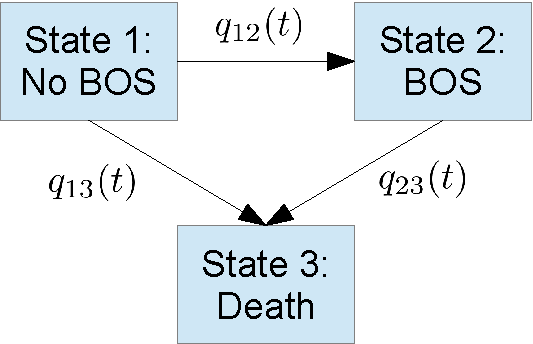
\includegraphics{bosmsm.pdf}}
  \caption{Three-state multi-state model for bronchiolitis obliterans syndrome (BOS)}
  \label{fig:bosmsm}
\end{figure}

\paragraph{Alternative time scales} 

In semi-Markov (clock-reset) models, $q_{rs}(t)$ depends on the time
$t$ since entry into the current state, but otherwise, the time since
the beginning of the process is forgotten.  Any software to fit
survival models can also fit this kind of multi-state model.

In an inhomogeneous Markov (clock-forward) model, $t$ represents the
time since the beginning of the process, but the intensity $q_{rs}(t)$
does not depend further on $\mathcal{H}_t$.  Again any survival
modelling software can be used, with the additional requirement that
it can deal with left-truncation or \emph{counting process} data.

These approaches are equivalent for competing risks models, since
there is at most one transition for each individual, so that the time
since the beginning of the process equals the time spent in the
current state.  Therefore no left-truncation is necessary.

\subsection{Representing multi-state data as survival data}

\citet{putter:mstate} discuss how to implement multi-state models by
manipulating the data into the a suitable form for survival modelling
software --- an overview is given here.  For each permitted $r
\rightarrow s$ transition in the multi-state model, there is a
corresponding ``survival'' (time-to-event) model, with hazard rates
defined by $q_{rs}(t)$.  For a patient who moves into state $r$ at
time $t_{j}$, their next event at $t_{j+1}$ is defined by the model
structure to be one of a set of competing events $s_1,\ldots,s_{n_r}$.
This implies there are $n_r$ corresponding survival models for this
state $r$, and $\sum_r n_r$ time-to-event models over all states $r$.
In the BOS example, there are $n_1=2,n_2=1$ and $n_3=0$ possible
transitions from states 1, 2 and 3 respectively.

The data to inform the $n_r$ models from state $r$ consists of an
indicator for whether the transition to the corresponding state
$s_1,\ldots,s_{n_r}$ is observed or censored at $t_{j+1}$, coupled
with:
\begin{itemize}
\item (for a semi-Markov model) the time elapsed $dt_{j} = t_{j+1} -
  t_{j}$ from state $r$ entry to state $s$ entry.  This data informs
  the ``survival'' model for the $r \rightarrow s$ transition.
  
\item (for an inhomogeneous Markov model) the start and stop time
  $(t_j,t_{j+1})$.  The $r \rightarrow s$ model is fitted to the
  right-censored time $t_{j+1}$ from the \emph{start of the process},
  but is conditional on not experiencing the $r \rightarrow s$
  transition until after the state $r$ entry time.  In other words,
  the $r \rightarrow s$ transition model is \emph{left-truncated} at
  the state $r$ entry time.
\end{itemize}

The \pkg{mstate} R package \citep{mstate:cmpb,mstate:jss} has a
utility \code{msprep} to produce data of this form from
``wide-format'' datasets where rows represent individuals, and times
of different events appear in different columns. \pkg{msm}
\citep{msmjss} has a similar utility \code{msm2Surv} for producing the
required form given longitudinal data where rows represent state
observations.

The outcomes of two patients in the BOS data are given by
\begin{Schunk}
\begin{Sinput}
> bosms3[18:22,]
\end{Sinput}
\begin{Soutput}
An object of class 'msdata'

Data:
   id from to    Tstart     Tstop     years status trans
18  7    1  2 0.0000000 0.1697467 0.1697467      1     1
19  7    1  3 0.0000000 0.1697467 0.1697467      0     2
20  7    2  3 0.1697467 0.6297057 0.4599589      1     3
21  8    1  2 0.0000000 8.1615332 8.1615332      0     1
22  8    1  3 0.0000000 8.1615332 8.1615332      1     2
\end{Soutput}
\end{Schunk}

Each row represents an observed (\code{status=1}) or censored
(\code{status=0}) transition time for one of three time-to-event
models indicated by the categorical variable \code{trans} (defined as
a factor).  Times are expressed in years, with the baseline time 0
representing six months after transplant.  Values of \code{trans} of
1, 2, 3 correspond to no BOS$\rightarrow$BOS, no BOS$\rightarrow$death
and BOS$\rightarrow$death respectively.  The first row indicates that
the patient (\code{id} 7) moved from state 1 (no BOS) to state 2 (BOS)
at 0.17 years, but (second row) this is also interpreted as a
censored time from state 1 to state 3, potential death before BOS
onset.  This patient then died, given by the third row with
\code{status} 1 for \code{trans} 3.  Patient 8 died before BOS onset,
therefore at 8.2 years their potential BOS onset is censored (fourth
row), but their death before BOS is observed (fifth row).

\subsection{Fitting parametric multi-state models}

Three multi-state models are fitted using \code{flexsurvreg}.  The
first two specified using the ``clock-reset'' time scale.  The first
is a simple time-homogeneous Markov model where all transition
intensities are constant through time, so that the clock-forward and
clock-reset scales are identical.  The time to the next event is
exponentially-distributed, but with a different rate $q_{rs}$ for each
transition type \code{trans}.  The second is a semi-Markov model where
the times to BOS onset, death without BOS and the time from BOS onset
to death all have Weibull distributions, with a different shape and
scale for each transition type.  The third is a clock-forward,
inhomogeneous Markov version of the Weibull model: the 1$\rightarrow$2
and 1$\rightarrow$3 transition models are the same, but the third has
a different interpretation, as the time \emph{from baseline} to death
with BOS has a Weibull distribution.
\begin{Schunk}
\begin{Sinput}
> crexp <- flexsurvreg(Surv(years, status) ~ trans, data=bosms3, 
+                      dist="exp")
> crwei <- flexsurvreg(Surv(years, status) ~ trans + shape(trans), 
+                      data=bosms3, dist="weibull")
> cfwei <- flexsurvreg(Surv(Tstart, Tstop, status) ~ trans + shape(trans), 
+                      data=bosms3, dist="weibull")
\end{Sinput}
\end{Schunk}
The equivalent Cox models are also fitted using
\code{coxph} from the \pkg{survival} package.  These specify a
different baseline hazard for each transition type through a function
\code{strata} in the formula, so since there are no other covariates,
they are essentially non-parametric.  Note that the \code{strata} function
is not currently understood by \code{flexsurvreg} --- the user must say
explicitly what parameters, if any, vary with the transition type,
as in \code{bwei}.
\begin{Schunk}
\begin{Sinput}
> crcox <- coxph(Surv(years, status) ~ strata(trans), data=bosms3)
> cfcox <- coxph(Surv(Tstart, Tstop, status) ~ strata(trans), data=bosms3)
\end{Sinput}
\end{Schunk}
In all cases, if there were other covariates, they could simply be
included in the model formula.  Typically, covariate effects will vary
with the transition type, so that an interaction term with
\code{trans} would be included.  Some post-processing might then be
needed to combine the main covariate effects and interaction terms
into an easily-interpretable quantity (such as the hazard ratio for
the $r,s$ transition).  Alternatively, \pkg{mstate} has a utility
\code{expand.covs} to expand a single covariate in the data into a set
of transition-specific covariates, to aid interpretation
\citep[see][]{mstate:jss}.

\subsection{Obtaining cumulative transition-specific hazards}

The \code{mstate} package enables \emph{semi-parametric} multi-state
modelling.  Models must be fitted with \code{coxph}, which also
provides a semi-parametric estimate of each transition-specific
baseline hazard \citep{mstate:cmpb,mstate:jss}.  These imply
piecewise-constant estimates of each cumulative $r \rightarrow s$
transition-specific hazard function $H_{rs}(t) = \int_0^t q_{rs}(u)
du$.  These estimates, and their covariances, are provided by
\pkg{mstate}'s function \code{msfit}, and form the basis of prediction
from the model.  For the Cox models for the BOS data,
\begin{Schunk}
\begin{Sinput}
> library(mstate)
> tmat <- rbind(c(NA,1,2),c(NA,NA,3),c(NA,NA,NA))
> mrcox <- msfit(crcox, trans=tmat)
> mfcox <- msfit(cfcox, trans=tmat)
\end{Sinput}
\end{Schunk}
\code{tmat} describes the transition structure.  This is a matrix of
integers whose $r,s$ entry is $i$ if the $i$th transition type is
$r,s$, and has \code{NA}s on the diagonal and where the $r,s$
transition is disallowed.

\pkg{flexsurv} provides an analogous function \code{msfit.flexsurvreg}
to produce cumulative hazards from \emph{fully-parametric} multi-state
models in the same format.  This is simply a wrapper around
\code{summary.flexsurvreg(...,type="cumhaz")}, as previously mentioned
in \S\ref{sec:plots}.  The difference from \pkg{mstate}'s method is
that hazard estimates can be produced for any grid of times \code{t},
at any level of detail and even beyond the range of the data, since
the model is fully parametric. The argument \code{newdata} can be used
in the same way to specify a desired covariate category, though in
this example there are no covariates in addition to the transition
type.  The name of the (factor) covariate indicating the transition
type can also be supplied through the \code{tvar} argument, in this
case it is the default, \code{"trans"}.
\begin{Schunk}
\begin{Sinput}
> tgrid <- seq(0,14,by=0.1)
> mrwei <- msfit.flexsurvreg(crwei, t=tgrid, trans=tmat)
> mrexp <- msfit.flexsurvreg(crexp, t=tgrid, trans=tmat)
> mfwei <- msfit.flexsurvreg(cfwei, t=tgrid, trans=tmat)
\end{Sinput}
\end{Schunk}
These can be plotted (Figure \ref{fig:bos:cumhaz}) to show the fit of
the parametric models compared to the non-parametric estimates.  Both
models appear to fit adequately, though give diverging extrapolations
after around 6 years when the data become sparse.  The Weibull
clock-reset model has an improved AIC of 1091, compared to
1099 for the exponential model.  For the 2--3 transition,
this shows that the clock forward and clock-reset models give slightly
different hazard trajectories.
\begin{figure}
\begin{Schunk}
\begin{Sinput}
> cols <- c("black","red","blue")
> plot(mrcox, xlab="Years after baseline", lwd=3, xlim=c(0,14), cols=cols)
> for (i in 1:3){
+     lines(tgrid, mrexp$Haz$Haz[mrexp$Haz$trans==i], col=cols[i], lty=2, lwd=2)
+     lines(tgrid, mrwei$Haz$Haz[mrwei$Haz$trans==i], col=cols[i], lty=3, lwd=2)
+ }
> lines(mfcox$Haz$time[mfcox$Haz$trans==3], mfcox$Haz$Haz[mfcox$Haz$trans==3],
+       type="s", col="darkgreen", lty=1, lwd=2)
> lines(tgrid, mfwei$Haz$Haz[mfwei$Haz$trans==3], col="darkgreen", lty=3, lwd=2)
> legend("topleft", inset=c(0,0.2), lwd=2, col=c("darkgreen"), 
+        c("2 -> 3 (clock-forward)"), bty="n")
> legend("topleft", inset=c(0,0.3), c("Non-parametric","Exponential","Weibull"),
+        lty=c(1,2,3), lwd=c(3,2,2), bty="n")
\end{Sinput}
\end{Schunk}
\includegraphics{flexsurv-032}
\caption{Cumulative hazards for three transitions in the BOS multi-state model, under non-parametric, exponential and Weibull models and clock-reset scales.  For the 2--3 transition, an alternative clock-forward scale is shown for the non-parametric and Weibull models.} 
\label{fig:bos:cumhaz}
\end{figure}

\subsection{Prediction from multi-state models}

Since \code{msfit.flexsurvreg} returns transition hazards in the same
format as \pkg{mstate}'s \code{msfit} method, the functions of
\pkg{mstate} for prediction can then be used.  For example, the
\emph{transition probabilities} of the multi-state model are the
probabilities of occupying each state $s$ at time $t > t_0$, given
that the individual is in state $r$ at time $t_0$.
\[ P(t_0, t) = P(S(t) = s | S(t_0) = r) \]
For an inhomogeneous Markov model, these are related to the transition
intensities via the Kolmogorov forward equation
\[ \frac{d P(t_0,t)}{dt} = P(t_0,t) Q(t) \] with initial condition
$P() = I$ \citep{cox:miller}.  An approximate solution
\citep[e.g.][]{aalen:process} is given by a product integral
\[ P(t_0, t) = \prod_{i=0}^{m-1} \left\{ I + Q(t_i) du \right\} \]
where a fine grid of times $t_0,t_1,\ldots,t_m=t$ is chosen to span
the prediction interval, and $Q(t_i) du$ is the increment in the
cumulative hazard matrix between times $t_i$ and $t_{i+1}$.  $Q$ may
also depend on other covariates, as long as these are known in
advance.

In \pkg{mstate} these can be calculated with the \code{probtrans}
function, applied to the cumulative hazards returned by \code{msfit}.
For Cox models, the time grid is naturally defined by the observed 
survival times, giving the
Aalen-Johansen estimator \citet{andersen}.  Here, the probability of
remaining alive and free of BOS is estimated at 0.27 at 5 years and 0.17
at 10 years.
\begin{Schunk}
\begin{Sinput}
> ptc <- probtrans(mfcox, predt=0, direction="forward")[[1]]
> ptc[c(165, 193),]
\end{Sinput}
\begin{Soutput}
        time   pstate1    pstate2   pstate3        se1        se2        se3
165 4.999316 0.2727122 0.29427877 0.4330090 0.03740559 0.03882367 0.04036366
193 9.872690 0.1740995 0.03975934 0.7861412 0.04031056 0.02224179 0.04462605
\end{Soutput}
\end{Schunk}
For parametric models, using a similar discrete-time approximation was
suggested by \citet{cook:lawless}.  This
is achieved by passing the object returned by \code{msfit.flexsurvreg}
to \code{probtrans} in \pkg{mstate}.  It can be made arbitrarily
accurate by choosing a finer resolution for the grid of times when 
calling \code{msfit.flexsurvreg}.  Under the Weibull model, the probability 
of remaining alive and free
of BOS is estimated at 0.3 at 5 years and 0.09 at 10 years: the
discrepancy from the Cox model is more marked at 10 years when the
data are more sparse (Figure~\ref{fig:bos:cumhaz}).
\begin{Schunk}
\begin{Sinput}
> ptw <- probtrans(mfwei, predt=0, direction="forward")[[1]]
> ptw[ptw$time %in% c(5,10),]
\end{Sinput}
\begin{Soutput}
    time    pstate1   pstate2   pstate3        se1        se2        se3
51     5 0.29984307 0.2543251 0.4458318 0.03454474 0.03482168 0.03850526
101   10 0.08853812 0.1194529 0.7920090 0.02925738 0.03241256 0.04301471
\end{Soutput}
\end{Schunk}
An alternative approach, not yet investigated in \pkg{flexsurv}, would
be to solve the Kolmogorov forward equation numerically, the approach
taken by \citet{titman:nonhomog}.

For semi-Markov models, these equations do not apply, since the
transition intensity matrix $Q(t)$ is not known in advance at time
$t$, but depends on when the transitions occur between time $t_0$ and
$t$.  $P(t_0, t)$ can then be estimated by simulation, given the
estimated cumulative hazards, using \pkg{mstate}'s function
\code{mssample} \citep{fiocco:mstatepred}.  5000 samples are
sufficient in this case to give estimates of transition probabilities
accurate to within around 0.01, and similar to the clock-forward
estimates.  Bootstrapping would be required for standard errors, which
would be computationally expensive given that it currently takes about
20 seconds to generate 5000 samples.
\begin{Schunk}
\begin{Sinput}
> mssample(mrcox$Haz, trans=tmat, clock="reset", M=5000, tvec=c(5, 10))
> mssample(mrwei$Haz, trans=tmat, clock="reset", M=5000, tvec=c(5, 10))
\end{Sinput}
\end{Schunk}




\subsection{Multi-state models for panel data}

Note the contrast between the models discussed in this section, and
multi-state models for \emph{panel data}, that is, observations of the
state of the process at a series of times \citep{kalbfleisch:lawless}.
In panel data, we do not necessarily know know the time of each
transition, or even whether transitions of a certain type have
occurred at all between a pair of observations.  Multi-state models
for this type of data (and also for the exact event time data
discussed above) can be fitted with the \pkg{msm} package for R
\citep{msmjss}, but are restricted to (piecewise)
exponentially-distributed event times.



\section{Potential extensions}
\label{sec:extensions}

Models where multiple survival times are assumed to be correlated
within groups, sometimes called (shared) frailty models
\citep{hougaard1995frailty}, would be a useful extension.  See,
e.g. \citet{crowther2014multilevel} for a recent application based on
parametric survival models.  These might be implemented by exploiting
tractability for specific distributions, such as gamma frailties, or
by adjusting standard errors to account for clustering, as implemented
in \code{survreg}.  More complex random effects models would require
numerical integration, and \citep{crowther2014multilevel} provide
Stata software based on Gauss-Hermite quadrature. Alternatively, a
probabilistic modelling language such as Stan \citep{stan-manual:2014}
or BUGS \citep{bugs:book} would be naturally suited to complex
extensions such as random effects on multiple parameters or multiple
hierarchical levels.

Relative survival models \citep{nelson:relative:survival}, often used
in cancer epidemiology, are a typical application of the Stata
packages mentioned in this article, but have not yet been attempted
with \pkg{flexsurv}.  These simply include an known additive offset in
the hazard function, representing the hazard for a reference
population, so would not be conceptually difficult.

\pkg{flexsurv} is intended as a platform for parametric survival
modelling.  Extensions of the software to deal with different models
may be written by users themselves, through the facilities described
in \S\ref{sec:custom} and \S\ref{sec:gdim}.  These might then be
included in the package as built-in distributions, or at least demonstrated
in the package's other vignette \code{flexsurv-examples}. Each
new class of models would ideally come with
\begin{itemize}
\item guidance on what situations the model is useful for, e.g. what
  shape of hazards it can represent

\item some intuitive interpretation of the model parameters, their
  plausible values in typical situations, and potential
  identifiability problems. This would also help with choosing initial
  values for numerical maximum likelihood estimation, ideally through
  an \code{inits} function in the custom distribution list
  (\S\ref{sec:custom}).
\end{itemize}

The examples in this paper were run using version 0.4 of \pkg{flexsurv}, available from \url{http://CRAN.R-project.org/package=flexsurv}.  Development versions are available on \url{https://github.com/chjackson/flexsurv-dev}, and contributions are welcome.

\appendix
\section{Acknowledgements}
Thanks to Milan Bouchet-Valat for help with implementing covariates on
ancillary parameters, Andrea Manca for motivating the development of
the package, and all users of the package who have reported bugs and
given suggestions.

\bibliography{flexsurv}

\end{document}
